% Compile twice with XeLaTeX. Figures are vector TikZ drawings in this file.
\documentclass[12pt]{article}
\usepackage[margin=1in]{geometry}
\usepackage{amsmath,amssymb,amsthm,microtype}
\usepackage[hidelinks]{hyperref}
\usepackage{fontspec}
\setmainfont{NewCM10-Book.otf}[BoldFont=NewCM10-Bold.otf,ItalicFont=NewCM10-BookItalic.otf,BoldItalicFont=NewCM10-BoldItalic.otf]
\usepackage{unicode-math}
\setmathfont{NewCMMath-Book.otf}
\usepackage[most]{tcolorbox}
\usepackage{tikz}
\usetikzlibrary{arrows.meta,patterns,calc}
\usepackage{booktabs,array,needspace}
\pretocmd{\section}{\Needspace{9\baselineskip}}{}{}
\pretocmd{\subsection}{\Needspace{7\baselineskip}}{}{}
\newtcolorbox{remarkbox}[1][Note]{colback=gray!5,colframe=gray!60,coltitle=black,title=#1,fonttitle=\bfseries,arc=2mm,boxrule=.6pt,breakable}
\newtcolorbox{todobox}[1]{colback=yellow!8,colframe=orange!75!black,title={TODO resolved: #1},fonttitle=\bfseries,arc=2mm,boxrule=.6pt,breakable}
\newtcolorbox{correctionbox}[1]{colback=red!3,colframe=red!55!black,title={Correction: #1},fonttitle=\bfseries,arc=2mm,boxrule=.6pt,breakable}
\newtcolorbox{conceptbox}[1]{colback=blue!3,colframe=blue!55!black,title={Supplement: #1},fonttitle=\bfseries,arc=2mm,boxrule=.6pt,breakable}
\newcommand{\E}{\mathbb E}
\newcommand{\Prob}{\mathbb P}
\newcommand{\R}{\mathbb R}
\newcommand{\ind}{\mathbf 1}
\DeclareMathOperator{\Var}{Var}
\DeclareMathOperator{\Lip}{Lip}
\DeclareMathOperator{\Law}{Law}
\setlength{\parindent}{0pt}
\setlength{\parskip}{5pt}
\allowdisplaybreaks
\tikzset{axis/.style={->,gray!80},pcurve/.style={blue!75!black,thick},qcurve/.style={orange!90!black,thick},every node/.style={font=\small}}
\title{STAT 581: Large Sample Theory\\\large Handwritten Notes 3, with an Illustrated Guide to Distances}
\author{Liang-Cheng Chen}
\date{October 19, 21, 26, and 28, 2026}
\newtcolorbox{gapbox}[1]{colback=cyan!4,colframe=cyan!50!black,title={Missing from original typed notes: #1},fonttitle=\bfseries,arc=2mm,boxrule=.6pt,breakable}
\begin{document}
\maketitle
\begin{remarkbox}[Sources and editorial conventions]
\raggedright
This English edited transcription covers all 31 pages of handwritten
\texttt{../notes/stat581-note3.pdf}, including the October 26 additions
on source pp. 21--31, together with the three substantive pages of
\texttt{stat581-note3 (2).pdf} (October 28; p. 4 is blank).
The first 20 pages were transcribed previously.
The reference is Yen-Chi Chen, \emph{Lecture 2: Introduction of large sample
 theory}, Autumn 2026, \texttt{Lec2\_large.pdf}.

Source-page labels refer to the handwritten PDF. Red boxes identify
mathematical corrections; yellow boxes preserve and answer the original five and four newly added explicit
TODOs, plus the two TODOs in the October 28 continuation; blue boxes add explanations. Appendix~\ref{sec:atlas} expands all seven
distance families in lecture Appendix B, with original vector diagrams.
The diagrams are explanatory examples, not claims about the source drawings.

All formulas use equation or align environments. There is no inline math:
TeX treats double-dollar delimiters as display math, not inline math.
\end{remarkbox}
\begin{remarkbox}[October 26 source comparison]
Cyan boxes identify omissions relative to the original typed version and give
teacher-source locations. Newly recovered classroom examples are ordinary
body text with source labels. Existing yellow, red, and blue boxes retain
their original meanings. The detailed audit is in \texttt{coverage-audit.md}.
The later October 26 handwriting update is integrated into the order-calculus
and delta-method sections. Source-page references there use the current
31-page student PDF; teacher-source references remain explicitly labeled.
\end{remarkbox}
\begingroup
\small
\tableofcontents
\endgroup
\clearpage

\section{Modes of convergence}
\subsection{Almost sure convergence and convergence in probability}
\textit{Source: pp. 1--2; lecture Definitions 2.1--2.2 and Theorem 2.4.}

Large sample theory studies sequences of random variables. The index may
represent sample size, an optimization iteration, or time. For almost sure
convergence and convergence in probability, the variables and their limit
are defined on a common probability space. For random vectors use the
Euclidean norm:
\begin{align}
 X_n\xrightarrow{\mathrm{a.s.}}Z
 &\quad\Longleftrightarrow\quad
 \Prob\!\left(\lim_{n\to\infty}\|X_n-Z\|=0\right)=1,\\
 X_n\xrightarrow{P}Z
 &\quad\Longleftrightarrow\quad
 \forall\varepsilon>0,\quad\Prob(\|X_n-Z\|>\varepsilon)\longrightarrow0.
\end{align}
Equivalently, convergence in probability says
\begin{equation}
 X_n-Z=o_P(1).
\end{equation}
This notation alone specifies no numerical rate. A concentration bound is
more quantitative; for example,
\begin{equation}
 \Prob(\|X_n-Z\|>\varepsilon)\le b(n,\varepsilon),
 \qquad b(n,\varepsilon)\longrightarrow0
 \quad\text{for every fixed }\varepsilon>0.
\end{equation}
The basic implications and uniqueness statements are
\begin{align}
 X_n\xrightarrow{\mathrm{a.s.}}Z&\ \Longrightarrow\ X_n\xrightarrow{P}Z,\\
 X_n\xrightarrow{\mathrm{a.s.}}Z,\quad X_n\xrightarrow{\mathrm{a.s.}}Y
 &\ \Longrightarrow\ \Prob(Z=Y)=1,\\
 X_n\xrightarrow{P}Z,\quad X_n\xrightarrow{P}Y
 &\ \Longrightarrow\ \Prob(Z=Y)=1.
\end{align}
\begin{conceptbox}{How Borel--Cantelli enters (source p. 1)}
A useful sufficient condition for almost sure convergence is
\begin{equation}
 \sum_{n=1}^{\infty}\Prob(\|X_n-Z\|>\varepsilon)<\infty
 \quad\text{for every }\varepsilon>0.
\end{equation}
Apply the first Borel--Cantelli lemma at reciprocal positive integers and
intersect the resulting probability-one events. Independence is unnecessary
for this direction. The second lemma requires independence (or an appropriate
replacement condition) to infer infinitely many occurrences from a divergent
sum; it is not needed for the typewriter example below.
\end{conceptbox}

\subsection{The typewriter counterexample}
\textit{Source: p. 2; lecture Example 2.3.}

Divide the unit interval into increasingly fine equal pieces, and let each
block of the sequence scan all pieces once:
\begin{align}
 U&\sim\operatorname{Unif}[0,1],\qquad
 N_{m,j}=\frac{m(m-1)}2+j,\quad 1\le j\le m,\\
 X_{N_{m,j}}&=\ind\!\left\{\frac{j-1}{m}\le U<\frac jm\right\}.
\end{align}
For any threshold strictly between zero and one, the exceedance probability
is the reciprocal block size:
\begin{equation}
 \Prob(X_{N_{m,j}}>\varepsilon)=\frac1m\longrightarrow0,
 \qquad 0<\varepsilon<1.
\end{equation}
Thus the sequence converges to zero in probability. For every realization
strictly below one, exactly one entry in each block equals one. There are
also infinitely many zeros, so almost sure convergence to zero fails.
The endpoint one is a null event.
\begin{correctionbox}{Indexing the blocks}
The handwritten second block reuses earlier indices. The triangular
indexing above removes that duplication while preserving the construction.
The probability of error vanishes, but a fixed sample path keeps encountering
errors. These are different statements.
\end{correctionbox}

\subsection{Consistency and convergence in distribution}
\textit{Source: pp. 3--4; lecture Definitions 2.5 and Theorems 2.6--2.7.}

An estimator is consistent when its estimation error tends to zero in
probability:
\begin{equation}
 \widehat\theta_n\xrightarrow{P}\theta
 \quad\Longleftrightarrow\quad
 \|\widehat\theta_n-\theta\|\xrightarrow{P}0.
\end{equation}
This does not by itself imply convergence of mean squared error. For example,
\begin{equation}
 \Prob(X_n=n^2)=\frac1n,\quad\Prob(X_n=0)=1-\frac1n
 \quad\Longrightarrow\quad
 X_n\xrightarrow{P}0,\qquad \E X_n^2=n^3.
\end{equation}
Convergence in distribution is convergence of laws, rather than closeness
of sample paths. In one dimension its CDF characterization is
\begin{equation}
 X_n\xrightarrow{d}Z
 \quad\Longleftrightarrow\quad
 F_{X_n}(t)\longrightarrow F_Z(t)
 \quad\text{at every continuity point of }F_Z.
\end{equation}
\begin{correctionbox}{The continuity-point qualification is essential}
Source p. 3 omits this qualification. At a jump of the limiting CDF, weak
convergence need not imply pointwise CDF convergence. The normal-to-point-mass
example in Section~\ref{sec:ks-source} makes this explicit.
\end{correctionbox}

The handwritten Portmanteau formulations are the following equivalent
conditions, in a fixed finite-dimensional Euclidean space:
\begin{align}
 &X_n\xrightarrow{d}Z;\\
 &\E f(X_n)\longrightarrow\E f(Z)
 \quad\text{for every bounded continuous }f;\\
 &\E f(X_n)\longrightarrow\E f(Z)
 \quad\text{for every bounded Lipschitz }f;\\
 &\E e^{it^{\mathsf T}X_n}\longrightarrow\E e^{it^{\mathsf T}Z}
 \quad\text{for every }t\in\R^d;\\
 &t^{\mathsf T}X_n\xrightarrow{d}t^{\mathsf T}Z
 \quad\text{for every }t\in\R^d.
\end{align}
The fourth line is L\'evy's continuity theorem; characteristic functions are
Fourier transforms of probability measures, which need not have densities.
The fifth is the Cram\'er--Wold device. Also,
\begin{align}
 X_n\xrightarrow{P}Z&\ \Longrightarrow\ X_n\xrightarrow{d}Z,\\
 X_n\xrightarrow{d}Z,\quad X_n\xrightarrow{d}Y
 &\ \Longrightarrow\ \Law(Z)=\Law(Y).
\end{align}
Uniqueness of the limiting law does not assert equality of the random
variables on a common sample space. Convergence in distribution to a
constant, however, does imply convergence in probability to that constant.

\begin{todobox}{N3-T1: A confidence interval and a test (source p. 3)}
Suppose independent identically distributed observations have finite mean
and positive finite variance. The CLT gives
\begin{equation}
 T_n=\frac{\sqrt n(\bar X_n-\mu)}{\sigma}\xrightarrow{d}N(0,1).
\end{equation}
Let the standard-normal quantile be defined by
\begin{equation}
 \Phi(z_{1-\alpha/2})=1-\alpha/2.
\end{equation}
Continuity of the normal CDF implies
\begin{equation}
 \Prob\!\left(\mu\in
 [\bar X_n-z_{1-\alpha/2}\sigma/\sqrt n,
  \bar X_n+z_{1-\alpha/2}\sigma/\sqrt n]\right)\longrightarrow1-\alpha.
\end{equation}
Under the null hypothesis that the mean equals a specified value, replacing
the mean in the pivot by that value gives a two-sided test: reject when the
absolute pivot exceeds this quantile. Its type-I error tends to the nominal
level. A consistent standard deviation estimate may replace the known
standard deviation by Slutsky's lemma.
\end{todobox}

\section{Distributional distances in the handwritten notes}
\textit{Source: pp. 5--7; lecture Appendix B, Definitions 2.36--2.44.}

Use probability measures for events and CDFs for one-dimensional threshold
probabilities. The three metrics that metrize weak convergence are
\begin{align}
 d_L(F,G)&=\inf\{\varepsilon>0:
 F(t-\varepsilon)-\varepsilon\le G(t)\le
 F(t+\varepsilon)+\varepsilon\ \text{for all }t\},\\
 d_{\mathrm{Pr}}(P,Q)&=\inf\{\varepsilon>0:
 P(A)\le Q(A^\varepsilon)+\varepsilon\ \text{for all Borel }A\},\\
 A^\varepsilon&=\{x:\inf_{y\in A}\|x-y\|<\varepsilon\},\\
 d_{\mathrm{BL}}(P,Q)&=\sup_{\|f\|_\infty\le1,\,\Lip(f)\le1}
 |\E_P f-\E_Q f|,\\
 \Lip(f)&=\sup_{x\ne y}\frac{|f(x)-f(y)|}{\|x-y\|},
 \qquad\|f\|_\infty=\sup_x|f(x)|.
\end{align}
Here the Prokhorov definition is the lecture's one-sided formulation; for
probability measures it is equivalent to imposing both directions. Appendix~\ref{sec:prok}
uses the symmetric formulation for its geometric explanation. L\'evy distance
applies to real-valued distributions; the other two apply on Euclidean spaces.
For a fixed real-valued limiting law,
\begin{equation}
 X_n\xrightarrow{d}Z
 \ \Longleftrightarrow\ d_L(F_{X_n},F_Z)\to0
 \ \Longleftrightarrow\ d_{\mathrm{Pr}}(P_{X_n},P_Z)\to0
 \ \Longleftrightarrow\ d_{\mathrm{BL}}(P_{X_n},P_Z)\to0.
\end{equation}
\begin{correctionbox}{A supremum, not an infimum (source pp. 5 and 7)}
The handwritten BL and Wasserstein dual formulas use an infimum over test
functions. That would always give zero, because the zero function is
admissible. The correct operation is the supremum: choose the test function
that best separates the two distributions. Wasserstein's transport
formulation instead uses an infimum over couplings.
\end{correctionbox}

Weak convergence does not control unbounded observables. The handwritten
contamination example can be written as
\begin{equation}
 P_n=\left(1-\frac1n\right)N(0,1)+\frac1n\delta_{n^2},
 \qquad P_n\Rightarrow N(0,1),\qquad \E_{P_n}X=n.
\end{equation}
Couple the mixture to a shared standard normal variable, replacing it only
on the contamination event. The discrepancy probability is at most the
mixture weight, so convergence in probability also holds, while the mean
diverges. Every bounded test function sees a discrepancy at most twice its
bound times that weight. Threshold indicators are bounded but not Lipschitz;
weak convergence controls them only at limiting CDF continuity points.

For laws with finite first absolute moments, the Wasserstein dual is
\begin{equation}
 W_1(P,Q)=\sup_{\Lip(f)\le1}|\E_P f-\E_Q f|.
\end{equation}
It removes the BL amplitude bound. The precise moment equivalence is
\begin{equation}\label{eq:w1conv}
 W_1(P_n,P)\to0
 \quad\Longleftrightarrow\quad
 P_n\Rightarrow P\ \text{and}\ \int\|x\|\,dP_n\to\int\|x\|\,dP.
\end{equation}
\begin{correctionbox}{Signed means are insufficient (source p. 7)}
Replace convergence of signed means by convergence of first absolute
moments. For example, the following laws have zero means and converge
weakly to a point mass, yet their Wasserstein distance does not vanish:
\begin{equation}
 P_n=(1-1/n)\delta_0+(1/2n)(\delta_n+\delta_{-n}),
 \qquad\E_{P_n}X=0,\quad W_1(P_n,\delta_0)=1.
\end{equation}
\end{correctionbox}
\begin{todobox}{N3-T2: BL intuition (source p. 5)}
A BL function is a measuring instrument with a bounded reading and bounded
slope. It cannot assign an arbitrarily large score to a tiny amount of
faraway mass, or change its reading abruptly across two nearby points.
Its worst possible expectation discrepancy measures weak convergence.
See the illustrated BL page in Appendix~\ref{sec:bl}.
\end{todobox}
\begin{todobox}{N3-T3: Why Wasserstein controls expectation (source p. 7)}
A linear coordinate function is Lipschitz but unbounded, so it is allowed
in the Wasserstein dual and excluded from the BL class. In one dimension,
\begin{equation}
 |\E_P X-\E_Q X|\le W_1(P,Q).
\end{equation}
The absolute-value function is also 1-Lipschitz, giving
\begin{equation}
 |\E_P|X|-\E_Q|X||\le W_1(P,Q).
\end{equation}
Thus vanishing transport cost forces both discrepancies to vanish.
The converse needs weak convergence and absolute moments as in
\eqref{eq:w1conv}; convergence of signed means alone is too weak.
\end{todobox}

\section{Moment convergence and transformations}
\subsection{Convergence in a moment norm}
\textit{Source: p. 8; lecture Definition 2.9 and Theorem 2.10.}

For a positive exponent, define moment convergence by
\begin{equation}
 X_n\xrightarrow{L^p}Z
 \quad\Longleftrightarrow\quad \E\|X_n-Z\|^p\to0.
\end{equation}
On a probability space, a larger moment controls a smaller one:
\begin{equation}
 s>p>0\quad\Longrightarrow\quad
 \bigl(\E\|X_n-Z\|^p\bigr)^{1/p}
 \le\bigl(\E\|X_n-Z\|^s\bigr)^{1/s}.
\end{equation}
Moreover, Markov's inequality gives
\begin{equation}
 \Prob(\|X_n-Z\|>\varepsilon)
 \le\frac{\E\|X_n-Z\|^p}{\varepsilon^p}\to0.
\end{equation}
This implication holds for every positive exponent, including those below
one (where the usual moment expression is not a norm). A limit in this
sense is unique almost surely. Squared moment convergence to a parameter
is exactly vanishing mean squared error.

\subsection{Continuous mapping and Slutsky's lemma}
\textit{Source: pp. 8--9; lecture Theorems 2.12--2.13.}

Suppose a measurable map is continuous at every point of a set receiving
probability one under the limiting variable. Applying it preserves each of
almost sure convergence, convergence in probability, and convergence in
distribution, respectively:
\begin{equation}
 X_n\xrightarrow{\star}Z\quad\Longrightarrow\quad
 f(X_n)\xrightarrow{\star}f(Z),
 \qquad \star\in\{\mathrm{a.s.},P,d\}.
\end{equation}
Slutsky's lemma combines a distributional limit with a constant probability
limit:
\begin{align}
 X_n\xrightarrow{d}Z,\quad Y_n\xrightarrow{P}c
 &\quad\Longrightarrow\quad X_n+Y_n\xrightarrow{d}Z+c,\\
 &Y_nX_n\xrightarrow{d}cZ\quad\text{when }Y_n\text{ is scalar},\\
 &X_n/Y_n\xrightarrow{d}Z/c\quad\text{when }Y_n\text{ is scalar and }c\ne0.
\end{align}
Addition requires matching dimensions. No independence assumption is needed.
The ratio assertion is central to studentization: a consistent positive
standard deviation estimate can replace the unknown population standard
deviation in a CLT pivot.

\section{Laws of large numbers and central limit theorems}
\subsection{The IID results}
\textit{Source: p. 10; lecture Theorems 2.14--2.15.}

For independent identically distributed observations, finite first absolute
moment gives the strong law, hence also the weak law:
\begin{equation}
 \E|X_1|<\infty\quad\Longrightarrow\quad
 \bar X_n\xrightarrow{\mathrm{a.s.}}\E X_1,
 \qquad\bar X_n\xrightarrow{P}\E X_1.
\end{equation}
For random vectors with finite second moment,
\begin{align}
 \mu&=\E X_1,\qquad\Sigma=\E[(X_1-\mu)(X_1-\mu)^{\mathsf T}],\\
 \E\|X_1\|^2<\infty
 &\quad\Longrightarrow\quad\sqrt n(\bar X_n-\mu)\xrightarrow{d}N_d(0,\Sigma).
\end{align}
A singular covariance is allowed; the limiting normal may be degenerate.
The right side of a convergence statement must be a fixed law, not a normal
law whose covariance still depends on the sample size.

\subsection{Triangular arrays: Lindeberg--Feller and Lyapunov}
\textit{Source: pp. 11--12 (October 21); lecture Theorem 2.17.}

For each row, let the observations be independent, without requiring
identical distributions or independence between rows:
\begin{align}
 X_{n,1},\ldots,X_{n,k_n},\qquad k_n&\longrightarrow\infty,\\
 \mu_{n,j}=\E X_{n,j},\quad\sigma_{n,j}^2&=\Var(X_{n,j})<\infty,\\
 s_n^2=\sum_{j=1}^{k_n}\sigma_{n,j}^2&>0,\qquad
 Y_{n,j}=\frac{X_{n,j}-\mu_{n,j}}{s_n}.
\end{align}
The denominator is the row's total standard deviation, not its total
variance. Either of the following sufficient conditions implies a normal
limit:
\begin{align}
 \text{Lindeberg:}\quad&
 \sum_{j=1}^{k_n}\E[Y_{n,j}^2\ind\{|Y_{n,j}|>\varepsilon\}]
 \longrightarrow0\quad\text{for every }\varepsilon>0;\\
 \text{Lyapunov:}\quad&
 \sum_{j=1}^{k_n}\E|Y_{n,j}|^{2+\delta}\longrightarrow0
 \quad\text{for some }\delta>0.
\end{align}
The conclusion is
\begin{equation}
 \sum_{j=1}^{k_n}Y_{n,j}\xrightarrow{d}N(0,1).
\end{equation}
Lyapunov implies Lindeberg because each truncated second moment is bounded
by the higher moment divided by the threshold to the extra power.
For an IID row with common positive variance and row length equal to the
sample size, the normalization becomes
\begin{equation}
 s_n=\sqrt n\sigma,\qquad
 \sum_{j=1}^nY_{n,j}=\frac{\sqrt n(\bar X_n-\mu)}{\sigma}.
\end{equation}
This framework also proves normality of regression estimators by expressing
them as weighted sums of independent errors. A design condition must ensure
no individual weighted observation dominates; the handwritten reference to
OLS is a motivation, not a proof for every design.

\section{Berry--Esseen, KS distance, and the bootstrap}
\subsection{A finite-sample normal approximation}
\textit{Source: pp. 13--14; lecture Appendix A, Theorem 2.34 (Berry--Esseen).}

For IID real observations, assume positive finite variance and a finite
third absolute centered moment. For some universal finite constant,
\begin{align}
 W_n&=\frac{\sqrt n(\bar X_n-\mu)}{\sigma},\qquad
 \rho_3=\E|X_1-\mu|^3<\infty,\\
 \sup_t|\Prob(W_n\le t)-\Phi(t)|
 &\le e_n:=\frac{C\rho_3}{\sigma^3\sqrt n}.
\end{align}
The bound holds at every sample size. It is informative when the bound is
small; a bound exceeding one is valid but uninformative.
\begin{correctionbox}{Center the third absolute moment (source p. 13)}
The source uses the uncentered third absolute moment without assuming a
zero mean. The standard Berry--Esseen expression uses the centered moment.
Finite uncentered third absolute moment is sufficient for its finiteness,
but the displayed numerical bound must use the correct quantity.
\end{correctionbox}

\begin{todobox}{N3-T4: Explain coverage and type-I error (source p. 14)}
For a one-sided normal critical value, the KS bound yields
\begin{equation}
 |\Prob(W_n\le z_{1-\alpha})-(1-\alpha)|\le e_n.
\end{equation}
Consequently, the upper confidence interval for the mean has coverage
within this error of the target:
\begin{equation}
 \Prob\!\left(\mu\le\bar X_n+z_{1-\alpha}\sigma/\sqrt n\right)
 \in[1-\alpha-e_n,1-\alpha+e_n].
\end{equation}
For the displayed upper interval apply the same KS bound at the negative
critical value; normal symmetry gives the stated target. Intersect bounds
with the unit interval when necessary. Similarly, rejecting the one-sided
null when the pivot exceeds the critical value gives type-I error within
the same error of the nominal level. A two-sided event uses two CDF
endpoints, so its coverage error is at most twice this bound.

These finite-sample bounds concern the known-variance pivot. Substituting
an estimated standard deviation preserves asymptotic validity under
consistency, but the same finite-sample bound does not follow from Slutsky
alone.
\end{todobox}

\subsection{KS versus weak convergence}\label{sec:ks-source}
\textit{Source: pp. 14--15; lecture Definitions 2.40 and Theorem 2.42.}
\begin{equation}
 d_{\mathrm{KS}}(F,G)=\sup_t|F(t)-G(t)|.
\end{equation}
KS convergence implies weak convergence. The converse holds if the fixed
limiting CDF is continuous everywhere (P\'olya's theorem).
\begin{todobox}{N3-T5: Weak convergence without KS convergence (source p. 15)}
Let the normal variance decrease to zero:
\begin{equation}
 X_n\sim N(0,1/n),\qquad X_n\xrightarrow{d}0,
 \qquad F_0(t)=\ind\{t\ge0\}.
\end{equation}
At zero the normal CDF is one half and the limiting CDF is one. Indeed,
\begin{equation}
 d_{\mathrm{KS}}(F_{X_n},F_0)=\frac12\quad\text{for every }n.
\end{equation}
The limiting CDF is discontinuous at zero, so P\'olya's continuity hypothesis
fails. Weak convergence correctly ignores this discontinuity point.
\end{todobox}

\subsection{Empirical bootstrap for the sample mean}
\textit{Source: pp. 16--17; lecture Appendix A.}

Given IID data with finite mean and positive variance, form the empirical law
and sample conditionally independently with replacement from it:
\begin{align}
 \widehat P_n&=\frac1n\sum_{i=1}^n\delta_{X_i},\qquad
 \widehat F_n(t)=\frac1n\sum_{i=1}^n\ind\{X_i\le t\},\\
 X_1^*,\ldots,X_n^*\mid X_1,\ldots,X_n
 &\overset{\mathrm{iid}}\sim\widehat P_n,\\
 \bar X_n^*&=\frac1n\sum_{i=1}^nX_i^*,\qquad
 \widehat\sigma_n^2=\frac1n\sum_{i=1}^n(X_i-\bar X_n)^2.
\end{align}
Bootstrap fluctuations about the observed mean approximate sampling
fluctuations about the population mean. Under a finite third absolute
moment, the rate statement in the handwriting has the rigorous form
\begin{equation}\label{eq:bootstrap}
 \sup_t\left|
 \Prob^*\!\left(\frac{\sqrt n(\bar X_n^*-\bar X_n)}{\widehat\sigma_n}\le t\right)
 -\Prob\!\left(\frac{\sqrt n(\bar X_n-\mu)}{\sigma}\le t\right)
 \right|=O_P(n^{-1/2}).
\end{equation}
Here the starred probability is conditional on the observed data. On the
rare event of zero empirical variance, define the starred pivot arbitrarily;
its probability tends to zero under the positive population variance assumption.

To see the rate, apply Berry--Esseen conditionally to the empirical law:
\begin{equation}
 \sup_t|\Prob^*(W_n^*\le t)-\Phi(t)|
 \le\frac{C\widehat\rho_{3,n}}{\widehat\sigma_n^3\sqrt n},
 \qquad\widehat\rho_{3,n}=\frac1n\sum_{i=1}^n|X_i-\bar X_n|^3.
\end{equation}
The empirical third centered moment is bounded in probability and the
empirical standard deviation converges to a positive constant. Apply the
ordinary Berry--Esseen bound to the unstarred pivot and use the triangle
inequality to obtain \eqref{eq:bootstrap}.
\begin{correctionbox}{What this bootstrap theorem says}
The source does not state its moment and nondegeneracy assumptions. They
are needed for the displayed rate. The second probability is a sampling
CDF, not itself ``the true CI coverage.'' Coverage follows only after
choosing an interval and relating its endpoints to the approximated CDF.
The bootstrap pivot above divides by the original empirical standard
deviation, not a newly computed standard deviation in every bootstrap sample.
\end{correctionbox}

\section{Deterministic and stochastic orders}
\textit{Source: pp. 17--20; lecture Section 2.5.}

For deterministic sequences with nonzero scaling terms eventually,
\begin{align}
 a_n=o(1)&\quad\Longleftrightarrow\quad a_n\to0,\\
 a_n=o(b_n)&\quad\Longleftrightarrow\quad a_n/b_n\to0,\\
 a_n=O(1)&\quad\Longleftrightarrow\quad
 \exists C<\infty,\ N:\ |a_n|\le C\ \text{for all }n\ge N,\\
 a_n=O(b_n)&\quad\Longleftrightarrow\quad a_n/b_n=O(1).
\end{align}
The constant must work for every sufficiently large index; choosing a
different unrestricted constant at every index would be vacuous.

For random sequences and positive deterministic scales, define
\begin{align}
 X_n=o_P(1)&\quad\Longleftrightarrow\quad X_n\xrightarrow{P}0,\\
 X_n=o_P(a_n)&\quad\Longleftrightarrow\quad X_n/a_n\xrightarrow{P}0,\\
 X_n=O_P(1)&\quad\Longleftrightarrow\quad
 \forall\varepsilon>0\ \exists M<\infty,\ N:
 \sup_{n\ge N}\Prob(\|X_n\|>M)<\varepsilon,\\
 X_n=O_P(a_n)&\quad\Longleftrightarrow\quad X_n/a_n=O_P(1).
\end{align}
Boundedness in probability concerns tails uniformly for sufficiently large
indices. It does not require a fixed almost sure bound. In finite-dimensional
Euclidean space it is equivalent to tightness of the sequence of laws;
the finitely many initial distributions do not affect this property.

A fixed Cauchy law also gives a tight sequence, despite having no finite
mean or variance. This classroom example (teacher handnotes October 21,
p.~9) emphasizes that stochastic boundedness is a tail-probability property,
not a moment assumption:
\begin{equation}
 X_n\sim\operatorname{Cauchy}(1,1)\quad\text{for every }n
 \quad\Longrightarrow\quad X_n=O_P(1).
\end{equation}

\subsection{Examples and nonuniqueness of rates}
\textit{Source: pp. 19--20.}
\begin{align}
 X_n\sim N(0,1/n)&\quad\Longrightarrow\quad X_n=O_P(n^{-1/2}),\\
 \E X_n=0,\quad\Var(X_n)=a_n^2
 &\quad\Longrightarrow\quad
 \Prob(|X_n|>Ma_n)\le M^{-2},\quad X_n=O_P(a_n).
\end{align}
A rate statement is an upper bound, not necessarily the sharpest rate.
For example,
\begin{align}
 X_n=o_P(1)&\ \Longrightarrow\ X_n=O_P(1),\\
 X_n=o_P(1)&\ \Longrightarrow\ X_n=o_P(n)\ \Longrightarrow\ X_n=O_P(n^2),\\
 X_n=O_P(1)&\ \Longrightarrow\ X_n=O_P(n)\ \Longrightarrow\ X_n=O_P(n^2).
\end{align}
Convergence in law implies boundedness in probability, and boundedness in
probability guarantees a weakly convergent subsequence:
\begin{align}
 X_n\xrightarrow{d}X&\quad\Longrightarrow\quad X_n=O_P(1),\\
 X_n=O_P(1)&\quad\Longrightarrow\quad
 \exists n_k\uparrow\infty,\ \exists P:\ \Law(X_{n_k})\Rightarrow P.
\end{align}
\begin{correctionbox}{A false converse (source p. 19)}
The handwritten equivalence between full-sequence weak convergence and
boundedness in probability must be a one-way implication. A deterministic
sequence alternating between zero and one is bounded, but its laws do not
converge. Its even and odd subsequences have different limits.
\end{correctionbox}
For IID observations with zero mean and positive finite variance, LLN and
CLT yield the final handwritten example:
\begin{equation}
 \bar X_n=o_P(1),\qquad
 \frac{\sqrt n\bar X_n}{\sigma}\xrightarrow{d}N(0,1),
 \qquad\bar X_n=O_P(n^{-1/2}).
\end{equation}
For a nonzero mean these statements apply to the centered sample mean.

\section{Additional Portmanteau formulations}
\begin{gapbox}{G2: the omitted set and semicontinuity criteria}
Lecture 2, Theorem 2.6, p. 2-3; teacher handnotes October 19, p. 6,
explicitly refers to additional lecture formulations. Original Notes 3
lists only the continuous-function, characteristic-function, and projection
versions. The lecture's item 7 has a typo: the set must be open.
\end{gapbox}
Weak convergence is equivalent to each of the following criteria:
\begin{align}
 \limsup_n\Prob(X_n\in C)&\le\Prob(Z\in C)
 &&\text{for every closed set }C,\\
 \liminf_n\Prob(X_n\in G)&\ge\Prob(Z\in G)
 &&\text{for every open set }G,\\
 \Prob(X_n\in A)&\to\Prob(Z\in A)
 &&\text{if }\Prob(Z\in\partial A)=0.
\end{align}
Equivalently, the limsup expectation inequality holds for every bounded
upper semicontinuous function, and the liminf inequality holds for every
bounded lower semicontinuous function. One-sided bounded versions also hold
with extended expectations interpreted appropriately.

For a concrete failure of probability convergence, take independent
standard normal variables on one common space:
\begin{equation}
 X_n\overset{\mathrm{iid}}\sim N(0,1),\quad Z\sim N(0,1)
 \text{ independent of all }X_n.
\end{equation}
All laws already equal the target law, but the difference has the same
nondegenerate normal law at every index, so it cannot converge to zero
in probability. This supplies the mechanism in lecture Example 2.8.

\section{Fixed-design regression as a triangular-array application}
\begin{gapbox}{G3: the OLS proof was only mentioned}
Lecture 2, Example 2.18, pp. 2-6--2-8; teacher handnotes October 21, p. 3.
The original Notes 3 gives the motivation but omits the design condition
and the proof. The following corrects transpose and normalization typos
in the lecture's derivation.
\end{gapbox}
For a fixed-dimensional full-rank design with row vectors, assume independent
identically distributed errors of mean zero and positive finite variance:
\begin{align}
 Y_n&=X_n\beta+e_n,\qquad\Var(e_i)=\sigma^2,\\
 \widehat\beta-\beta&=(X_n^{\mathsf T}X_n)^{-1}X_n^{\mathsf T}e_n,\\
 a_{n,i}&=(X_n^{\mathsf T}X_n)^{-1/2}x_{n,i},\qquad
 \sum_i a_{n,i}a_{n,i}^{\mathsf T}=I_p.
\end{align}
A sufficient no-dominant-observation condition is vanishing maximum leverage:
\begin{equation}
 \max_i h_{n,ii}=\max_i\|a_{n,i}\|^2\to0.
\end{equation}
For a fixed nonzero vector, the normalized scalar summands have total
variance one. Their Lindeberg sum is bounded by a common tail second moment:
\begin{align}
 b_{n,i}&=\frac{t^{\mathsf T}a_{n,i}}{\|t\|},\quad
 \sum_i b_{n,i}^2=1,\quad m_n=\max_i|b_{n,i}|\to0,\\
 \sum_i\E\left[\frac{b_{n,i}^2e_i^2}{\sigma^2}
 \mathbf1\{|b_{n,i}e_i|>\varepsilon\sigma\}\right]
 &\le\frac1{\sigma^2}\E[e_1^2\mathbf1\{|e_1|>\varepsilon\sigma/m_n\}]
 \to0.
\end{align}
Cram\'er--Wold therefore gives
\begin{equation}
 (X_n^{\mathsf T}X_n)^{1/2}(\widehat\beta-\beta)
 \xrightarrow{d}N_p(0,\sigma^2 I_p).
\end{equation}
If the normalized Gram matrix tends to a positive definite matrix, then
\begin{equation}
 n^{-1}X_n^{\mathsf T}X_n\to Q>0
 \quad\Longrightarrow\quad
 \sqrt n(\widehat\beta-\beta)\xrightarrow{d}N_p(0,\sigma^2Q^{-1}).
\end{equation}
Symmetry of the error law is unnecessary. Finite variance and the design
condition supply the needed Lindeberg control.

\section{Stochastic-order calculus and sample variance}
\begin{gapbox}{G4: order algebra and a worked variance estimator}
Lecture 2, Proposition 2.25 and Examples 2.26--2.28, pp. 2-10--2-11,
were absent from the original typed notes and supplied teacher handnotes.
The updated student notes now cover these topics on pp. 21--27.
\end{gapbox}
\textit{Student source: pp. 21--27, October 26; lecture Proposition 2.25
and Examples 2.26--2.28.}

\subsection{Stochastic algebra and all eight mixed relations}
The six handwritten rules on p. 21 are, with no independence required,
\begin{align}
 o_P(1)+o_P(1)&=o_P(1),& O_P(1)+O_P(1)&=O_P(1),\\
 O_P(1)+o_P(1)&=O_P(1),& O_P(1)o_P(1)&=o_P(1),\\
 [1+o_P(1)]^{-1}&=1+o_P(1),& o_P(1)&\subseteq O_P(1).
\end{align}
The inverse therefore is bounded in probability, but does not converge to
zero. Define it arbitrarily on any vanishing-probability event where its
denominator is zero. The notation describes classes of sequences: repeated
order symbols need not denote the same random remainder.

\begin{todobox}{Complete the eight relations (source p. 22)}
For deterministic small/bounded sequences and random small/tight sequences,
Lecture 2 Proposition 2.25 gives all four sums and all four products:
\begin{align}
 o_P(1)+o(1)&=o_P(1),& o_P(1)+O(1)&=O_P(1),\\
 O_P(1)+o(1)&=O_P(1),& O_P(1)+O(1)&=O_P(1),\\
 o_P(1)o(1)&=o_P(1),& o_P(1)O(1)&=o_P(1),\\
 O_P(1)o(1)&=o_P(1),& O_P(1)O(1)&=O_P(1).
\end{align}
The blank lines in the handwriting do not specify an ordering; the completed
list follows the lecture. The mnemonic ``drop P, do algebra, restore P''
helps recall these rules, but the definitions justify them.
\end{todobox}
For example, a product of a tight factor and a factor converging to zero
converges to zero because, for any positive threshold and cutoff,
\begin{equation}
 \Prob(|U_nV_n|>\varepsilon)
 \le \Prob(|U_n|>M)+\Prob(|V_n|>\varepsilon/M).
\end{equation}
First choose the cutoff to control the tight factor, then take the sample
size large. Independence is unnecessary. For positive deterministic scales,
\begin{align}
 O_P(a_n)+O_P(b_n)&=O_P(a_n+b_n),\\
 O_P(a_n)O_P(b_n)&=O_P(a_nb_n),\\
 o_P(a_n)O_P(b_n)&=o_P(a_nb_n),\\
 [c+o_P(1)]^{-1}&=c^{-1}+o_P(1),\qquad c\ne0.
\end{align}

\subsection{What an order statement does not imply}
\textit{Student source: pp. 23 and 27.}
Deterministic bounds and bounds in probability differ. The exact classroom
example is
\begin{equation}
 X_n\sim N(0,n^{-2}),\quad a_n=1,\qquad
 X_n+a_n\sim N(1,n^{-2}),\qquad X_n+a_n=O_P(1).
\end{equation}
Every finite-sample law has unbounded support, so there is no deterministic
uniform bound over all possible outcomes. It nevertheless converges to one
in probability. In fact a common coupling can even be almost surely
eventually bounded; that is distinct from a deterministic bound.

The second handwritten example is
\begin{equation}
 X_n\sim
 \begin{cases}N(0,1),&n\text{ even},\\
 \operatorname{Unif}[-1,1],&n\text{ odd}.
 \end{cases}
\end{equation}
This sequence is tight, but its two subsequences have different laws, so
there is no full-sequence weak limit. Nor does tightness control moments:
a fixed Cauchy law has no finite mean, while the rare-spike example gives
\begin{equation}
 \Prob(X_n=n^2)=1/n,\quad \Prob(X_n=0)=1-1/n,
 \qquad X_n\xrightarrow{P}0,\quad \E X_n=n\to\infty.
\end{equation}
These are different failures: undefined moments versus diverging finite
moments. An order bound alone rules out neither.

\subsection{Density estimation: bias, variability, and bandwidth}
\begin{todobox}{Supply the KDE versus histogram example (source pp. 23--24)}
The handwriting requests a bias--variability decomposition and sketches
small Gaussian kernels placed at the observations. No worked teacher
example is present in the supplied teacher PDFs. The following is an
editorial completion, with the assumptions stated explicitly.
\end{todobox}
Let the observations be IID with density, and consider a fixed evaluation
point and a deterministic bandwidth:
\begin{align}
 \widehat p_h(x)&=\frac1{nh}\sum_{i=1}^n
 K\!\left(\frac{x-X_i}{h}\right),\\
 \widehat p_h(x)-p(x)
 &=\{\E\widehat p_h(x)-p(x)\}
   +\{\widehat p_h(x)-\E\widehat p_h(x)\}.
\end{align}
Assume the density is bounded and globally Lipschitz, the kernel is
nonnegative and integrates to one, and the following integrals are finite:
\begin{align}
 \int |u|K(u)\,du&<\infty,\qquad R(K)=\int K(u)^2\,du<\infty,\\
 |\E\widehat p_h(x)-p(x)|
 &\le Lh\int |u|K(u)\,du=O(h),\\
 \Var(\widehat p_h(x))&\le\frac{\|p\|_\infty R(K)}{nh}.
\end{align}
Chebyshev's inequality yields precisely the requested pointwise rate:
\begin{equation}
 \widehat p_h(x)-p(x)=O(h)+O_P((nh)^{-1/2}),
 \qquad h\to0,\quad nh\to\infty.
\end{equation}
For a fixed histogram bin of width equal to the bandwidth and containing
the evaluation point, the same Lipschitz assumption gives
\begin{align}
 \widehat p_{\mathrm{hist}}(x)&=
 \frac1{nh}\sum_i\ind\{X_i\in B_h(x)\},\\
 |\E\widehat p_{\mathrm{hist}}(x)-p(x)|&\le Lh,\qquad
 \Var(\widehat p_{\mathrm{hist}}(x))\le\frac{\|p\|_\infty}{nh}.
\end{align}
Thus the two estimators share this conservative rate. Balancing the two
terms suggests a bandwidth of order the inverse cube root of sample size
and a pointwise error of that same order. The histogram is piecewise
constant; Gaussian KDE is smooth.

\begin{conceptbox}{When a symmetric kernel improves the bias}
If the density has a bounded continuous second derivative, a symmetric
kernel with finite second moment cancels the first-order term:
\begin{align}
 \mu_2(K)&=\int u^2K(u)\,du,\qquad \int uK(u)\,du=0,\\
 \E\widehat p_h(x)-p(x)&=
 \tfrac12 h^2\mu_2(K)p''(x)+o(h^2),\\
 \widehat p_h(x)-p(x)&=O(h^2)+O_P((nh)^{-1/2}).
\end{align}
Balancing now suggests a bandwidth of order the inverse fifth root of
sample size and pointwise error of order the inverse two-fifths power.
These are pointwise statements; boundaries and uniform errors require
additional analysis. The original first-order bias is valid under its
weaker smoothness assumption, rather than a universal sharp KDE rate.
\end{conceptbox}

\subsection{Sample variance: expand the remainders, state the assumptions}
\textit{Student source: pp. 25--27.}
The red handwritten reminder says to work backward from the desired result,
identify each theorem, and check its assumptions before applying it. Here,
IID observations with finite fourth moment allow a CLT for the empirical
second moment as well as the mean. Write
\begin{align}
 \mu&=\E X_1,\quad m_2=\E X_1^2,\quad \sigma^2=m_2-\mu^2,\\
 M_n&=n^{-1}\sum_iX_i^2=m_2+R_{2n},\qquad R_{2n}=O_P(n^{-1/2}),\\
 \bar X_n&=\mu+R_{1n},\qquad R_{1n}=O_P(n^{-1/2}),\\
 \bar X_n^2&=\mu^2+2\mu R_{1n}+R_{1n}^2,\qquad
 R_{1n}^2=O_P(n^{-1}),\\
 M_n-\bar X_n^2
 &=\sigma^2+R_{2n}-2\mu R_{1n}-R_{1n}^2
 =\sigma^2+O_P(n^{-1/2}),\\
 S_n^2&=\frac{n}{n-1}(M_n-\bar X_n^2)
       =\sigma^2+O_P(n^{-1/2}).
\end{align}
The two first-order random remainders are absorbed into the same order;
they are not canceled. The extra normalization contributes only a term
of order the reciprocal sample size, because the bracket is tight.
Finite second moment alone suffices for consistency by LLN; finite fourth
moment is sufficient for the displayed rate. Simulation can illustrate
the rate but does not replace checking these hypotheses.

\begin{conceptbox}{Connection to a one-step estimator (source p. 26, NOTE)}
The variance expansion is already asymptotically linear:
\begin{align}
 S_n^2-\sigma^2&=\frac1n\sum_i\{(X_i-\mu)^2-\sigma^2\}
                  +O_P(n^{-1}),\\
 \sqrt n(S_n^2-\sigma^2)&\xrightarrow{d}
 N\!\left(0,\E(X_1-\mu)^4-\sigma^4\right).
\end{align}
This is the same first-order idea used in a one-step correction. For a
smooth scalar estimating equation with nonzero population derivative,
its Newton update from a preliminary estimate is
\begin{align}
 \Psi_n(t)&=n^{-1}\sum_i\psi(X_i,t),\\
 \widehat\theta_{\mathrm{one}}
 &=\widetilde\theta-\{\dot\Psi_n(\widetilde\theta)\}^{-1}
                         \Psi_n(\widetilde\theta).
\end{align}
With a consistent empirical derivative and controlled second derivatives,
a preliminary error smaller than the inverse fourth root of sample size
makes its quadratic Taylor remainder negligible on the root-sample-size
scale. These are additional regularity requirements; order notation alone
does not guarantee a valid one-step procedure. The variance identity above
is exact up to an explicitly controlled remainder, without a Newton step.
\end{conceptbox}

\subsection{Gaussian concentration gives more than a stochastic order}
\textit{Student source: p. 27, ``MGF + Markov's: how?''}
For IID centered normal observations with positive variance, both bounds
below imply the usual sample-mean order:
\begin{align}
 \Prob(|\bar X_n|>\varepsilon)&\le\frac{\sigma^2}{n\varepsilon^2},\\
 \Prob(|\bar X_n|>\varepsilon)&\le
 2\exp\!\left(-\frac{n\varepsilon^2}{2\sigma^2}\right),\\
 \bar X_n&=O_P(n^{-1/2}).
\end{align}
For the exponential bound, use the Gaussian moment generating function
and Markov's inequality, for any positive tuning parameter:
\begin{align}
 \E e^{t\bar X_n}&=\exp(t^2\sigma^2/(2n)),\\
 \Prob(\bar X_n>\varepsilon)&\le
 \exp(-t\varepsilon+t^2\sigma^2/(2n)).
\end{align}
Minimize at the threshold times sample size divided by the variance and
apply the same argument to the negative sample mean. The handwritten
constant is therefore the reciprocal of twice the population variance.
Substituting a cutoff times the inverse square root of sample size gives
\begin{equation}
 \Prob(\sqrt n|\bar X_n|>M)\le
 \min\{\sigma^2/M^2,\,2e^{-M^2/(2\sigma^2)}\}.
\end{equation}
Both bounds can be made arbitrarily small by increasing the cutoff,
which proves stochastic boundedness. At a fixed positive threshold the
exponential bound decays much faster in sample size. Stochastic order
alone suppresses that quantitative distinction.

\section{Delta method and asymptotic linearity}
\begin{gapbox}{G5: all of Lecture 2 Section 2.6 was missing}
Lecture 2, Theorems 2.29--2.31 and Examples 2.30--2.32, pp. 2-11--2-14.
The updated student notes cover this material on pp. 28--31; it is not
in the supplied teacher handnotes through October 21.
The lecture's displayed conclusions omit the rate multiplier; its rate
sequence must diverge, rather than decrease.
\end{gapbox}
\textit{Student source: pp. 28--31; lecture Theorems 2.29--2.31.}

Suppose a diverging deterministic rate yields a limiting distribution and
the transformation is differentiable at the target:
\begin{align}
 r_n&\to\infty,\qquad r_n(W_n-\omega_0)\xrightarrow{d}Z,\\
 f(W_n)-f(\omega_0)&=J_f(\omega_0)(W_n-\omega_0)+o_P(r_n^{-1}),\\
 r_n\{f(W_n)-f(\omega_0)\}&\xrightarrow{d}J_f(\omega_0)Z.
\end{align}
The proof writes the deterministic differentiability remainder as an
error of order smaller than the input norm, uses consistency to make
its coefficient small in probability, and tightness to bound the scaled
input. For a normal limit the covariance transforms to
\begin{equation}
 J_f(\omega_0)\Sigma J_f(\omega_0)^{\mathsf T}.
\end{equation}
\begin{conceptbox}{Vector delta method and Jacobian dimensions (source p. 28)}
For an input in a finite-dimensional Euclidean space and a vector-valued
map, the Jacobian has one row per output and one column per input:
\begin{align}
 W_n,\omega_0&\in\R^d,\quad f:\R^d\to\R^k,
 \quad J_f(\omega_0)\in\R^{k\times d},\\
 r_n(W_n-\omega_0)&\xrightarrow{d}N_d(0,\Sigma),\\
 r_n\{f(W_n)-f(\omega_0)\}&\xrightarrow{d}
 N_k\!\left(0,J_f(\omega_0)\Sigma J_f(\omega_0)^{\mathsf T}\right).
\end{align}
For scalar output the gradient is a column, so its transpose is the
Jacobian. The handwritten gradient-transpose covariance formula and the
Jacobian formula above are the same convention expressed differently.
\end{conceptbox}
For exponential observations with rate parameter, the reciprocal sample
mean has limit
\begin{equation}
 \sqrt n(\bar X_n-\lambda^{-1})\xrightarrow{d}N(0,\lambda^{-2})
 \quad\Longrightarrow\quad
 \sqrt n(\bar X_n^{-1}-\lambda)\xrightarrow{d}N(0,\lambda^2).
\end{equation}
If the first derivative vanishes, first-order delta gives a degenerate
limit; a higher-order expansion may be needed. For example,
\begin{equation}
 \sqrt nW_n\xrightarrow{d}N(0,\sigma^2)
 \quad\Longrightarrow\quad nW_n^2\xrightarrow{d}\sigma^2\chi_1^2.
\end{equation}
The last example is an editorial exercise, not a stated lecture theorem.

An asymptotically linear estimator has the representation
\begin{equation}
 \widehat\theta_n-\theta_0=\frac1n\sum_i\psi(X_i)+o_P(n^{-1/2}),
 \qquad\E\psi(X_1)=0,\quad\E\|\psi(X_1)\|^2<\infty.
\end{equation}
Its asymptotic covariance is the covariance of its influence function.
For a transformed empirical mean the influence function is the Jacobian
times the centered summand, not its uncentered second moment.

\subsection{Relative risk: cell proportions, covariance, and inference}
\textit{Student source: pp. 29--30; lecture Example 2.32.}
Assume IID binary observation pairs and equal treatment probabilities.
The handwritten target is a ratio conditional on observing an outcome:
\begin{align}
 \Prob(T=1)&=\Prob(T=0)=1/2,\qquad (T,Y)\in\{0,1\}^2,\\
 \theta&=\frac{\Prob(T=1\mid Y=1)}{\Prob(T=0\mid Y=1)}
 =\frac{\Prob(T=1,Y=1)}{\Prob(T=0,Y=1)}.
\end{align}
The outcome probability cancels in this expression. By Bayes' rule and
equal allocation, it also equals the usual outcome risk ratio:
\begin{equation}
 \theta=\frac{\Prob(Y=1\mid T=1)}{\Prob(Y=1\mid T=0)}.
\end{equation}
Without equal allocation, the ratio of joint cells differs from that risk
ratio by the allocation odds. Define the cell indicators and proportions:
\begin{align}
 \zeta_{ty}&=\Prob(T=t,Y=y),\qquad
 a=\zeta_{11}>0,\quad b=\zeta_{01}>0,\\
 A_i&=T_iY_i,\qquad B_i=(1-T_i)Y_i,\\
 A_n&=n^{-1}\sum_i A_i,\qquad B_n=n^{-1}\sum_i B_i,
 \qquad\widehat\theta_n=A_n/B_n,\quad\theta=a/b.
\end{align}
The positive denominator assumption ensures the estimator is defined with
probability tending to one; set it arbitrarily when no denominator cell
is observed. For the nondegenerate log and Wald formulas below we also
assume a positive numerator cell probability.

\begin{todobox}{What are the entries of the covariance matrix? (source p. 29)}
The cell indicators are Bernoulli, and their product is identically zero:
\begin{align}
 \Var(A_i)&=a(1-a),&\Var(B_i)&=b(1-b),\\
 A_iB_i&=0,&\operatorname{Cov}(A_i,B_i)&=-ab,\\
 \Sigma&=\begin{pmatrix}a(1-a)&-ab\\-ab&b(1-b)\end{pmatrix}.
\end{align}
The off-diagonal entries are equal by symmetry of covariance. Disjoint
cells are not independent: the negative covariance is essential.
\end{todobox}
\begin{correctionbox}{Center the vector before applying the CLT (source p. 29)}
The handwriting scales the uncentered vector. The correct statement is
\begin{equation}
 \sqrt n\left\{\begin{pmatrix}A_n\\B_n\end{pmatrix}
              -\begin{pmatrix}a\\b\end{pmatrix}\right\}
 \xrightarrow{d}N_2(0,\Sigma).
\end{equation}
Without centering, the scaled mean vector diverges because its population
cell probabilities are positive.
\end{correctionbox}
For the ratio map, the gradient and the delta-method variance are
\begin{align}
 f(x,y)&=x/y,\qquad
 \nabla f(x,y)=\begin{pmatrix}1/y\\-x/y^2\end{pmatrix},\\
 \sqrt n(\widehat\theta_n-\theta)&\xrightarrow{d}N(0,V),\\
 V&=\nabla f(a,b)^{\mathsf T}\Sigma\nabla f(a,b)
 =\frac{a}{b^2}+\frac{a^2}{b^3}
 =\frac{\theta(1+\theta)}b.
\end{align}
A consistent plug-in variance and an asymptotic Wald interval are
\begin{align}
 \widehat V_n&=\frac{A_n}{B_n^2}+\frac{A_n^2}{B_n^3},\\
 \widehat\theta_n&\ \mathbin{\pm}\ z_{1-\alpha/2}\sqrt{\widehat V_n/n}.
\end{align}
A log-scale interval stays positive after exponentiation:
\begin{align}
 \sqrt n\{\log\widehat\theta_n-\log\theta\}
 &\xrightarrow{d}N(0,1/a+1/b),\\
 \text{interval}&=\exp\!\left\{\log\widehat\theta_n
 \mathbin{\pm}z_{1-\alpha/2}\sqrt{(1/A_n+1/B_n)/n}\right\}.
\end{align}
These approximations require positive observed cell proportions; they can
be poor for sparse cells at a finite sample size.

\subsection{Modern approach: expand the ratio directly}
\begin{todobox}{Finish the teacher-note expansion (source p. 31)}
The handwriting stops after substituting population values plus errors.
Write the errors and apply the inverse expansion:
\begin{align}
 \Delta_{1n}&=A_n-a=O_P(n^{-1/2}),\\
 \Delta_{0n}&=B_n-b=O_P(n^{-1/2}),\\
 \widehat\theta_n
 &=\frac{a+\Delta_{1n}}{b+\Delta_{0n}},\\
 (b+\Delta_{0n})^{-1}
 &=b^{-1}-b^{-2}\Delta_{0n}+O_P(n^{-1}),\\
 \widehat\theta_n-\theta
 &=\frac{\Delta_{1n}}b-\frac{a\Delta_{0n}}{b^2}+O_P(n^{-1}).
\end{align}
The inverse remainder follows, on a neighborhood of the positive
population denominator, from the exact identity
\begin{equation}
 \frac1{b+d}=\frac1b-\frac{d}{b^2}+\frac{d^2}{b^2(b+d)}.
\end{equation}
Products of two root-sample-size errors have reciprocal-sample-size
order and disappear after multiplication by the square root of sample
size. Applying the multivariate CLT to the remaining linear terms recovers
the same variance as the delta method.
\end{todobox}
The corresponding influence function makes the cancellation transparent:
\begin{align}
 \psi(T_i,Y_i)&=\frac{A_i-a}{b}-\frac{a(B_i-b)}{b^2}
              =\frac{A_i}{b}-\frac{aB_i}{b^2},\\
 \E\psi(T_i,Y_i)&=0,\qquad \Var\{\psi(T_i,Y_i)\}=V,\\
 \widehat\theta_n-\theta&=n^{-1}\sum_i\psi(T_i,Y_i)+O_P(n^{-1}).
\end{align}
Here the population constants really cancel algebraically; generic
stochastic-order symbols in the earlier variance calculation do not.


\subsection{October 28 continuation: exact remainders and unequal rates}
\textit{Student continuation: \texttt{stat581-note3 (2).pdf}, pp. 1--3;
lecture reference: Lecture 2, delta-method and ratio-estimator discussion.}
The first continuation page repeats the unfinished expansion on original
source p. 31. The October 28 pages then subtract the population ratio and
expand the inverse denominator. Use the same cell means as above, and set
\begin{equation}
 d_{1n}=A_n-a,\qquad d_{0n}=B_n-b,\qquad b>0.
\end{equation}
These are the handwritten numerator and denominator errors, respectively.
The population cell probabilities are fixed; the errors shrink in probability.
\begin{todobox}{Complete the teacher-note calculation (continuation p. 1)}
An exact subtraction is more informative than an order symbol:
\begin{align}
 \frac{A_n}{B_n}-\frac ab
 &=\frac{d_{1n}}b-\frac{a\,d_{0n}}{b^2}+R_n,\\
 R_n&=-\frac{d_{1n}d_{0n}}{b(b+d_{0n})}
       +\frac{a\,d_{0n}^2}{b^2(b+d_{0n})}.
\end{align}
On an event whose probability tends to one, the denominator is bounded
away from zero. Consequently, for deterministic positive rate sequences,
\begin{align}
 d_{1n}&=O_P(r_n),\quad d_{0n}=O_P(s_n),\quad r_n,s_n\longrightarrow0,\\
 R_n&=O_P(r_ns_n+s_n^2).
\end{align}
This finishes the requested calculation using the lecture's linearization
principle. The exact identity and the unequal-rate formulation are editorial
explanations, rather than a transcription of additional teacher handwriting.
\end{todobox}
\begin{correctionbox}{Do not discard the denominator-square term (continuation p. 3)}
The handwritten remainder retains only the product of the two errors.
In general the squared denominator error is also present. For example,
if the numerator error is identically zero and the numerator mean is
nonzero, the exact remainder above is still nonzero. Under root-sample-size
rates both terms have the same upper order, so the final root-sample-size
normal limit in the notes remains valid:
\begin{equation}
 d_{1n},d_{0n}=O_P(n^{-1/2})\quad\Longrightarrow\quad
 R_n=O_P(n^{-1})=o_P(n^{-1/2}).
\end{equation}
Also write errors with deterministic rate bounds, rather than using a random
error itself as the scale in an ambiguous stochastic-order expression.
\end{correctionbox}
For the ordering of errors used on handwritten p. 3, the CLT and variance are
\begin{align}
 \sqrt n\begin{pmatrix}d_{0n}\\d_{1n}\end{pmatrix}
 &\xrightarrow{d}N_2(0,\Sigma_{01}),\\
 c&=\begin{pmatrix}-a/b^2\\1/b\end{pmatrix},\qquad
 \sqrt n(\widehat\theta_n-\theta)\xrightarrow{d}
 N(0,c^{\mathsf T}\Sigma_{01}c).
\end{align}
Reversing the coordinate order requires reversing the corresponding rows,
columns, and gradient entries. This is the same variance derived above.

\begin{todobox}{Why use this argument instead of the delta method? (continuation p. 3)}
For ordinary IID cell proportions, the multivariate delta method is shorter
and gives exactly the same result. The direct expansion exposes each error
and its remainder, which is helpful when the numerator and denominator
have different convergence rates, or when nuisance functions are estimated.
If a common deterministic scaling has a joint limit and negligible remainder,
\begin{align}
 t_n(d_{1n},d_{0n})^{\mathsf T}&\xrightarrow{d}Z,\\
 t_n(r_ns_n+s_n^2)&\longrightarrow0,\\
 t_n(\widehat\theta_n-\theta)&\xrightarrow{d}
 b^{-1}Z_1-ab^{-2}Z_2.
\end{align}
The limit need not be Gaussian. Different rates alone do not guarantee a
CLT; a joint limit for the relevant linear term is still needed. A generalized
delta-method argument can also handle these scales.
\end{todobox}
\begin{conceptbox}{The AIPW/IPW marginal note}
The handwriting mentions AIPW and IPW as motivation for tracking rates.
For a generic ratio, the algebra above gives both the product and square
remainders. In an orthogonal AIPW estimating equation, an additional
structural cancellation can instead produce a product of two nuisance
estimation errors. For example, errors with reciprocal-fourth-root rates
whose product is little-oh of the reciprocal square root can be negligible
at the root-sample-size scale. This requires overlap, suitable moment
bounds, and empirical-process control (often obtained by sample splitting);
it is not an automatic property of every ratio or IPW estimator.
\end{conceptbox}

\section{Bootstrap consistency with only a second moment}
\begin{gapbox}{G6: the conditional triangular-array proof}
Lecture 2, Appendix A.1, pp. 2-14--2-16. Original Notes 3 gives only
the stronger third-moment Berry--Esseen argument.
\end{gapbox}
Under a positive finite variance, conditionally on the observations,
\begin{equation}
 \mathcal L^*\{\sqrt n(\bar X_n^*-\bar X_n)\}
 \Rightarrow N(0,\sigma^2)\quad\text{almost surely}.
\end{equation}
Here is the key tail step behind conditional Lindeberg. For any fixed
positive threshold and any fixed truncation level, eventually
\begin{align}
 \frac1n\sum_i X_i^2\mathbf1\{|X_i|>\varepsilon\sqrt n\}
 &\le\frac1n\sum_i X_i^2\mathbf1\{|X_i|>K\},\\
 \limsup_n\frac1n\sum_i X_i^2\mathbf1\{|X_i|>\varepsilon\sqrt n\}
 &\le\E[X_1^2\mathbf1\{|X_1|>K\}]\longrightarrow0
 \quad(K\to\infty).
\end{align}
Centering by the sample mean does not alter this conclusion because the
sample mean converges to a finite constant. Conditional total variance
converges to the population variance by LLN. Apply the triangular-array
CLT on probability-one sample paths, then P\'olya's theorem for the
continuous normal limit to obtain conditional KS consistency. This proves
convergence without the third-moment rate. It does not assert an automatic
rate for every bootstrap confidence interval.

\clearpage
\appendix
\section{Illustrated distributional distances}\label{sec:atlas}
\textit{Editorial supplement based on lecture Appendix B, pp. 2-17--2-23.}

Each distance asks a different question about two probability laws. For
real-valued variables write their CDFs as follows:
\begin{equation}
 F(t)=P(({-\infty},t]),\qquad G(t)=Q(({-\infty},t]).
\end{equation}
L\'evy and KS use the CDF directly; Prokhorov uses neighborhoods of events;
BL and Wasserstein use test functions or transport; TV and Hellinger use
probability mass or density geometry. Every figure below illustrates a
definition or an exactly computable example.

\subsection{L\'evy: allow horizontal and vertical CDF error}\label{sec:levy}
\begin{equation}
 d_L(F,G)=\inf\{\varepsilon>0:
 F(t-\varepsilon)-\varepsilon\le G(t)
 \le F(t+\varepsilon)+\varepsilon\ \text{for all }t\}.
\end{equation}
\textbf{Intuition.} Enclose one CDF between shifted copies of the other.
Horizontal slack allows nearby locations to count as similar; vertical
slack tolerates a small probability discrepancy. Both use the same numerical
budget, so the value depends on the units of the horizontal axis.

\begin{center}
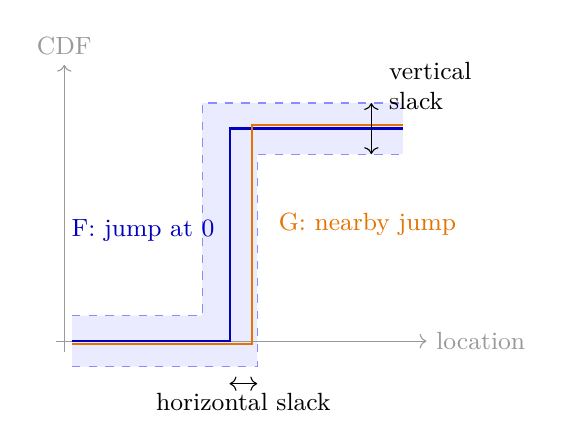
\begin{tikzpicture}[x=1cm,y=2.7cm]
 \fill[blue!8] (-2,.12) -- (-.35,.12) -- (-.35,1.12) -- (2.2,1.12) -- (2.2,.88) -- (.35,.88) -- (.35,-.12) -- (-2,-.12) -- cycle;
 \draw[axis] (-2.2,0)--(2.5,0) node[right]{location};
 \draw[axis] (-2.1,-.05)--(-2.1,1.3) node[above]{CDF};
 \draw[blue!45,dashed] (-2,.12)--(-.35,.12)--(-.35,1.12)--(2.2,1.12);
 \draw[blue!45,dashed] (-2,-.12)--(.35,-.12)--(.35,.88)--(2.2,.88);
 \draw[pcurve] (-2,0)--(0,0)--(0,1)--(2.2,1);
 \draw[qcurve] (-2,-.015)--(.28,-.015)--(.28,1.015)--(2.2,1.015);
 \node[blue!75!black] at (-1.1,.52){F: jump at 0};
 \node[orange!90!black,right] at (.5,.55){G: nearby jump};
 \draw[<->] (0,-.2)--(.35,-.2) node[midway,below]{horizontal slack};
 \draw[<->] (1.8,.88)--(1.8,1.12);
 \node[right,align=left] at (1.9,1.2){vertical\\slack};
\end{tikzpicture}
\end{center}
\textit{Figure A.1.} Blue dashed curves form a horizontal-and-vertical
slack envelope around a unit step. The orange step lies inside the envelope.
Horizontal and vertical scales are intentionally different for legibility.

\textbf{Exact example.} Moving a unit point mass by a nonnegative displacement gives
\begin{equation}
 d_L(\delta_0,\delta_h)=\min\{h,1\},\qquad h\ge0.
\end{equation}
A small shift is cheap even though the CDF jumps. This is why the metric
can go to zero at a discontinuous limiting law. For a fixed limiting law
on the real line, vanishing L\'evy distance is equivalent to weak convergence.

\clearpage
\subsection{Prokhorov: enlarge an event and allow missing mass}\label{sec:prok}
\begin{align}
 A^\varepsilon&=\{x:d(x,A)<\varepsilon\},\\
 d_{\mathrm{Pr}}(P,Q)=\inf\{\varepsilon>0:\quad
 P(A)&\le Q(A^\varepsilon)+\varepsilon,\quad
 Q(A)\le P(A^\varepsilon)+\varepsilon
 \ \text{for every Borel }A\}.
\end{align}
\textbf{Intuition.} Before comparing an event's probability, expand its
boundary by the spatial budget. Then allow an additional probability
budget of unmatched mass. This accommodates both small spatial errors and
rare large errors.

\begin{center}
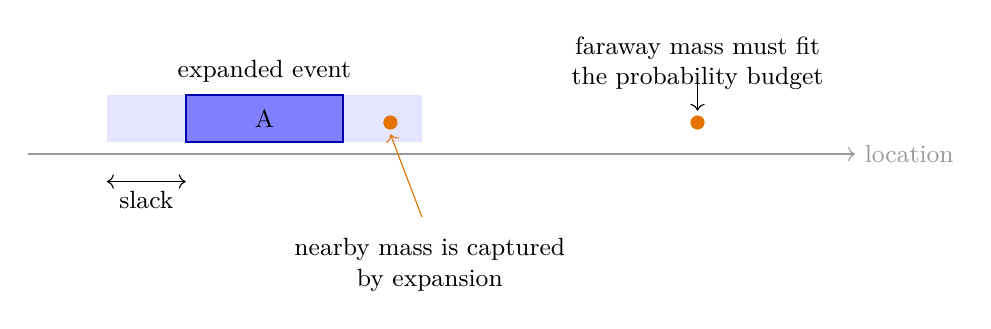
\begin{tikzpicture}[x=1cm,y=1cm]
 \draw[axis] (-.5,0)--(10,0) node[right]{location};
 \fill[blue!10] (.5,.15) rectangle (4.5,.75);
 \fill[blue!50] (1.5,.15) rectangle (3.5,.75);
 \draw[blue!70!black,thick] (1.5,.15) rectangle (3.5,.75);
 \node at (2.5,.45){A};
 \node at (2.5,1.05){expanded event};
 \draw[<->] (.5,-.35)--(1.5,-.35) node[midway,below]{slack};
 \fill[orange!90!black] (4.1,.4) circle (.09);
 \node[align=center,anchor=north] at (4.6,-.95){nearby mass is captured\\by expansion};
 \draw[->,orange!90!black] (4.5,-.8)--(4.1,.25);
 \fill[orange!90!black] (8,.4) circle (.09);
 \node[align=center] at (8,1.15){faraway mass must fit\\the probability budget};
 \draw[->] (8,.9)--(8,.55);
\end{tikzpicture}
\end{center}
\textit{Figure A.2.} A set and its open neighborhood. The nearby orange point
is recovered geometrically; the distant point must be accounted for as
unmatched probability.

\textbf{Coupling interpretation.} On a Euclidean space, this metric is the
infimum of budgets for which a coupling of the two laws can satisfy
\begin{equation}
 \Prob(\|X-Y\|>\varepsilon)\le\varepsilon,
 \qquad X\sim P,\quad Y\sim Q.
\end{equation}
Strict versus non-strict inequalities at the boundary do not change the
infimum. This does not require the originally observed variables to have
this joint distribution; one may choose any coupling.

For point masses and a contamination example,
\begin{align}
 d_{\mathrm{Pr}}(\delta_0,\delta_h)&=\min\{|h|,1\},\\
 Q=(1-a)\delta_0+a\delta_M
 &\quad\Longrightarrow\quad d_{\mathrm{Pr}}(\delta_0,Q)\le a,
 \qquad 0\le a\le1.
\end{align}
A rare outlier is cheap regardless of how far away it lies. The metric
metrizes weak convergence in Euclidean spaces; it does not impose moment
convergence.

\clearpage
\subsection{Bounded Lipschitz: limited range and slope}\label{sec:bl}
\begin{equation}
 d_{\mathrm{BL}}(P,Q)=
 \sup_{\|f\|_\infty\le1,\,\Lip(f)\le1}|\E_P f-\E_Q f|.
\end{equation}
\textbf{Intuition.} Let an observer choose a scoring function. The function
may change by at most the distance between inputs and must stay between
minus one and one. The best observer's expected-score gap is the distance.
Both constraints matter: slope limits sensitivity to nearby shifts; range
limits sensitivity to distant outliers.

\begin{center}
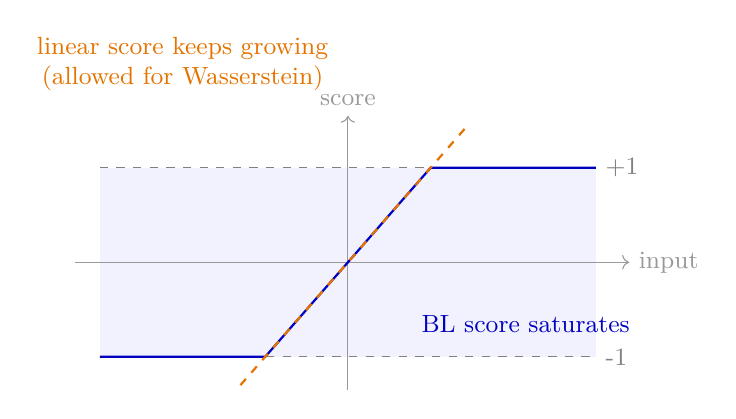
\begin{tikzpicture}[x=1.05cm,y=1.2cm]
 \fill[blue!5] (-3,-1) rectangle (3,1);
 \draw[axis] (-3.3,0)--(3.4,0) node[right]{input};
 \draw[axis] (0,-1.35)--(0,1.55) node[above]{score};
 \draw[gray,dashed] (-3,1)--(3,1) node[right]{+1};
 \draw[gray,dashed] (-3,-1)--(3,-1) node[right]{-1};
 \draw[pcurve] (-3,-1)--(-1,-1)--(1,1)--(3,1);
 \draw[orange!90!black,dashed,thick] (-1.3,-1.3)--(1.45,1.45);
 \node[blue!75!black,align=center] at (2.15,-.65){BL score saturates};
 \node[orange!90!black,align=center] at (-2,2.1){linear score keeps growing\\(allowed for Wasserstein)};
\end{tikzpicture}
\end{center}
\textit{Figure A.3.} The clipped identity is a valid BL score. The unbounded
identity satisfies the slope constraint but fails the BL range constraint.

For two point masses the optimal score can use the full difference between
minus one and one:
\begin{equation}
 d_{\mathrm{BL}}(\delta_x,\delta_y)=\min\{\|x-y\|,2\}.
\end{equation}
For a small mixture perturbation,
\begin{equation}
 Q=(1-a)P+aR
 \quad\Longrightarrow\quad d_{\mathrm{BL}}(P,Q)\le2a.
\end{equation}
The factor two comes from the possible difference of two scores in the
allowed range. In particular, a bad event with vanishing probability
cannot prevent BL convergence even if its magnitude explodes.

\begin{remarkbox}[Definition convention]
We follow the lecture's separate range and slope bounds. Some books instead
bound the sum of these two quantities by one. These conventions induce the
same weak convergence, but numerical distances and comparison constants
can differ. A supremum over the full fixed class is stronger than checking
one chosen score; both characterize weak convergence when used correctly.
\end{remarkbox}

\clearpage
\subsection{Kolmogorov--Smirnov: the worst threshold-probability error}
\begin{equation}
 d_{\mathrm{KS}}(F,G)=\sup_t|F(t)-G(t)|
 =\sup_t|P(X\le t)-Q(Y\le t)|.
\end{equation}
\textbf{Intuition.} Place a threshold anywhere on the number line. Compare
the probability to its left under the two laws. KS is the largest vertical
CDF gap; there is no permission to shift the threshold horizontally.

\begin{center}
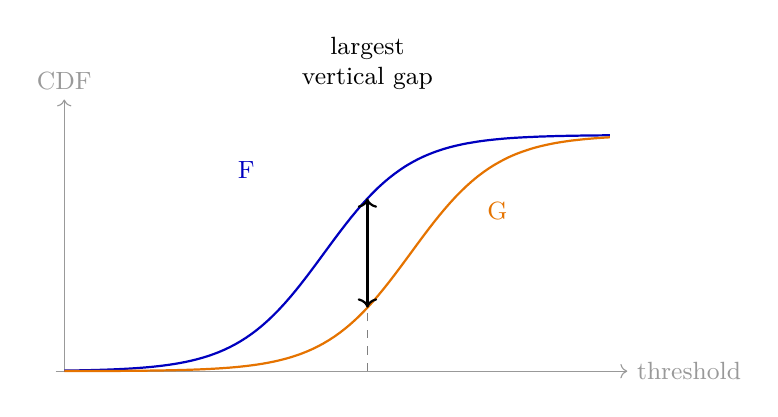
\begin{tikzpicture}[x=1.1cm,y=3cm]
 \draw[axis] (-3.1,0)--(3.5,0) node[right]{threshold};
 \draw[axis] (-3,0)--(-3,1.15) node[above]{CDF};
 \draw[pcurve,domain=-3:3.3,samples=100] plot (\x,{1/(1+exp(-2*\x))});
 \draw[qcurve,domain=-3:3.3,samples=100] plot (\x,{1/(1+exp(-2*(\x-1)))});
 \draw[<->,thick] (.5,.269)--(.5,.731);
 \draw[gray,dashed] (.5,0)--(.5,.269);
 \node[above,align=center] at (.5,1.15){largest\\vertical gap};
 \node[blue!75!black] at (-.9,.85){F};
 \node[orange!90!black] at (2,.68){G};
\end{tikzpicture}
\end{center}
\textit{Figure A.4.} Two logistic CDFs shifted by one unit. The maximum
vertical separation occurs halfway between their centers.

KS bounds directly control probability error for a one-sided event. For an
interval, subtract two CDFs, giving at most twice the KS error. This explains
its role in Berry--Esseen bounds and confidence interval coverage.

An arbitrarily small shift of a point mass gives
\begin{equation}
 d_{\mathrm{KS}}(\delta_0,\delta_h)=1\quad(h\ne0),
 \qquad d_L(\delta_0,\delta_h)\to0\quad(h\to0).
\end{equation}
A threshold placed between the two atoms separates them perfectly. Hence
KS is strictly stronger than weak convergence in general. At a fixed
continuous limiting CDF, P\'olya's theorem makes the two convergence criteria
equivalent. This is an asymptotic statement, not a universal numerical bound
between the two distances.

\clearpage
\subsection{Wasserstein: minimum transport cost}
For a real exponent at least one and laws with finite corresponding moments,
\begin{equation}
 W_p(P,Q)=\inf_{\pi\in\Pi(P,Q)}
 \left(\int\|x-y\|^p\,d\pi(x,y)\right)^{1/p}.
\end{equation}
\textbf{Intuition.} Treat probability as divisible material. A transport
plan specifies how much mass goes from each origin to each destination.
Choose the plan with least average powered distance, then take the root.
The joint law is a coupling; it may split mass and need not be a deterministic
transport map. Larger powers penalize long moves more heavily.

\begin{center}
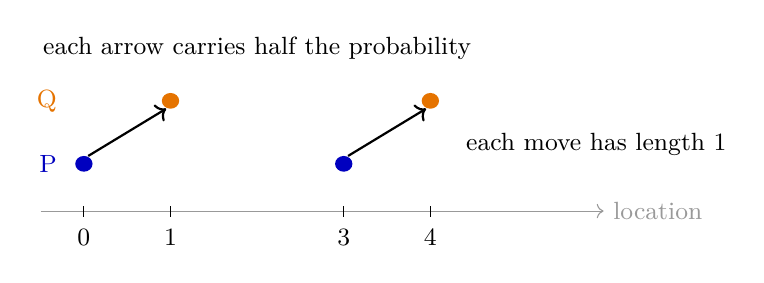
\begin{tikzpicture}[x=1.1cm,y=1cm]
 \draw[axis] (-.5,0)--(6,0) node[right]{location};
 \foreach \x/\lab in {0/0,1/1,3/3,4/4}{\draw (\x,-.07)--(\x,.07);\node[below] at (\x,-.1){\lab};}
 \fill[blue!75!black] (0,.6) circle (.1);\fill[blue!75!black] (3,.6) circle (.1);
 \fill[orange!90!black] (1,1.4) circle (.1);\fill[orange!90!black] (4,1.4) circle (.1);
 \draw[->,thick] (.05,.7)--(.95,1.3);
 \draw[->,thick] (3.05,.7)--(3.95,1.3);
 \node[left,blue!75!black] at (-.2,.6){P};\node[left,orange!90!black] at (-.2,1.4){Q};
 \node[above] at (2,1.8){each arrow carries half the probability};
 \node[right] at (4.3,.85){each move has length 1};
\end{tikzpicture}
\end{center}
\textit{Figure A.5.} Equal masses at zero and three move to one and four.
The monotone matching is optimal in one dimension, and every Wasserstein
distance with exponent at least one equals one in this example.

In one dimension the common-quantile coupling is optimal:
\begin{align}
 F^{-1}(u)&=\inf\{x:F(x)\ge u\},\qquad 0<u<1,\\
 W_p^p(P,Q)&=\int_0^1|F^{-1}(u)-G^{-1}(u)|^p\,du,\\
 W_1(P,Q)&=\int_{\R}|F(t)-G(t)|\,dt
 =\sup_{\Lip(f)\le1}|\E_Pf-\E_Qf|.
\end{align}
Thus KS measures the tallest CDF gap, whereas one-dimensional Wasserstein
with exponent one measures the \emph{area} between CDFs. For a rare outlier,
\begin{equation}
 Q=(1-a)\delta_0+a\delta_M
 \quad\Longrightarrow\quad W_p(\delta_0,Q)=a^{1/p}|M|.
\end{equation}
Unlike BL or Prokhorov, Wasserstein charges for how far the outlier travels.
Its convergence criterion in Euclidean space is
\begin{equation}
 W_p(P_n,P)\to0\quad\Longleftrightarrow\quad
 P_n\Rightarrow P\ \text{and}\
 \int\|x\|^p\,dP_n\to\int\|x\|^p\,dP<\infty.
\end{equation}
\textbf{Distinguish two notions.} Moment convergence of given random variables
uses their actual joint law; Wasserstein minimizes over all joint laws.
Thus moment convergence implies Wasserstein convergence of the laws, but
the converse need not hold for the original coupling.
Uniform integrability is another route from weak convergence to moment
convergence; using a Wasserstein metric is not mandatory.

\clearpage
\subsection{Total variation: the best event for distinguishing two laws}
For densities with respect to a common dominating measure,
\begin{align}
 p&=\frac{dP}{d\lambda},\qquad q=\frac{dQ}{d\lambda},\\
 d_{\mathrm{TV}}(P,Q)&=\sup_{A\ \mathrm{Borel}}|P(A)-Q(A)|\\
 &=\frac12\int|p-q|\,d\lambda
 =1-\int\min(p,q)\,d\lambda.
\end{align}
\textbf{Intuition.} Choose \emph{any} measurable event to maximize the
probability gap. A maximizing event is the region where the first density
exceeds the second. The distance is the probability mass left over after
overlapping as much of the two laws as possible. It ignores spatial distance.

\begin{center}
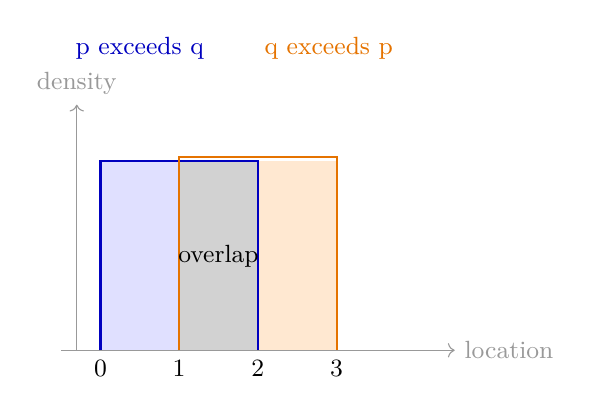
\begin{tikzpicture}[x=1cm,y=2.4cm]
 \fill[gray!35] (1,0) rectangle (2,1);
 \fill[blue!12] (0,0) rectangle (1,1);
 \fill[orange!18] (2,0) rectangle (3,1);
 \draw[axis] (-.5,0)--(4.5,0) node[right]{location};
 \draw[axis] (-.3,0)--(-.3,1.3) node[above]{density};
 \draw[pcurve] (0,0)--(0,1)--(2,1)--(2,0);
 \draw[qcurve] (1,0)--(1,1.025)--(3,1.025)--(3,0);
 \node at (1.5,.5){overlap};
 \node[blue!75!black,align=center] at (.5,1.6){p exceeds q};
 \node[orange!90!black,align=center] at (2.9,1.6){q exceeds p};
 \foreach \x in {0,1,2,3}{\node[below] at (\x,0){\x};}
\end{tikzpicture}
\end{center}
\textit{Figure A.6.} Uniform laws on the intervals from zero to two and from
one to three. Both density heights are one half; the drawing rescales the
vertical axis. The overlap has mass one half, so TV equals one half.
The orange top edge is offset slightly to show both curves.

\textbf{Testing interpretation.} If either law is equally likely a priori,
the minimum average probability of classification error is
\begin{equation}
 R_{\mathrm{test}}^*=\frac{1-d_{\mathrm{TV}}(P,Q)}2.
\end{equation}
Zero TV means the laws cannot be distinguished; TV equal to one means
there is a measurable event that perfectly distinguishes them. Under an
optimal coupling, TV is also the minimum probability that the two coupled
variables are unequal.

A point mass moved by any nonzero amount has TV equal to one, even if the
move is tiny. By contrast, a contamination of size one percent changes any
event probability by at most one percent:
\begin{equation}
 d_{\mathrm{TV}}(P,(1-a)P+aR)\le a.
\end{equation}
A density with respect to Lebesgue measure is unnecessary: taking the
dominating measure to be the sum of the two probability laws always works.
This covers discrete, continuous, and mixed distributions uniformly.

\clearpage
\begingroup\small
\subsection{Hellinger: square-root density geometry}
We use the normalized convention from lecture Definition 2.51:
\begin{align}
 H^2(P,Q)&=\frac12\int(\sqrt p-\sqrt q)^2\,d\lambda
 =1-\rho(P,Q),\\
 \rho(P,Q)&=\int\sqrt{pq}\,d\lambda,\qquad 0\le H(P,Q)\le1.
\end{align}
\textbf{Intuition.} Taking the square root of a density maps every law to
a unit vector in an inner-product space. Affinity is the inner product of
the two unit vectors. Hellinger distance is their Euclidean chord length
divided by the square root of two, not the angular or arc distance.

\begin{center}
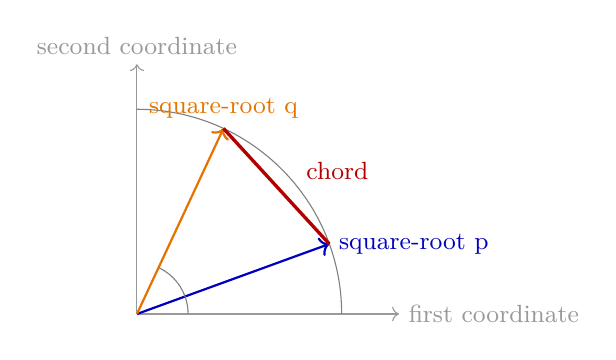
\begin{tikzpicture}[scale=2.6]
 \draw[axis] (0,0)--(1.28,0) node[right]{first coordinate};
 \draw[axis] (0,0)--(0,1.22) node[above]{second coordinate};
 \draw[gray] (1,0) arc (0:90:1);
 \draw[->,pcurve] (0,0)--({cos(20)},{sin(20)});
 \draw[->,qcurve] (0,0)--({cos(65)},{sin(65)});
 \draw[red!70!black,very thick] ({cos(20)},{sin(20)})--({cos(65)},{sin(65)});
 \draw[gray] (.25,0) arc (0:65:.25);
 \node[right,blue!75!black] at ({cos(20)},{sin(20)}){square-root p};
 \node[above,orange!90!black] at ({cos(65)},{sin(65)}){square-root q};
 \node[red!70!black,right] at (.78,.7){chord};
\end{tikzpicture}
\end{center}
\textit{Figure A.7.} For two-point distributions, square-root probability
vectors lie on the positive quadrant of a unit circle. General densities
have the same geometry in an infinite-dimensional function space.

For Bernoulli laws, the formula is explicit:
\begin{equation}
 H^2(\operatorname{Ber}(a),\operatorname{Ber}(b))
 =1-\sqrt{ab}-\sqrt{(1-a)(1-b)}.
\end{equation}
Affinity multiplies across independent observations, so
\begin{equation}
 H^2(P^{\otimes n},Q^{\otimes n})=1-\rho(P,Q)^n
 =1-(1-H^2(P,Q))^n.
\end{equation}
This makes Hellinger useful for likelihood theory and testing lower bounds.
In a regular differentiable parametric family, a small parameter displacement
has the local Fisher-information approximation
\begin{equation}
 H^2(P_{\theta+h},P_\theta)
 =\frac18h^{\mathsf T}I(\theta)h+o(\|h\|^2).
\end{equation}
This approximation requires quadratic-mean differentiability; it is not an
identity valid for every family.

\begin{correctionbox}{Hellinger normalization in the lecture}
Definition 2.51 uses the normalized convention above. The upper TV bound
in Theorem 2.52 and the product formula in Appendix B.4 mix conventions.
With this document's convention the consistent formulas are
\begin{equation}
 H^2\le d_{\mathrm{TV}}\le H\sqrt{2-H^2},\qquad
 H^2(P^{\otimes n},Q^{\otimes n})=1-(1-H^2(P,Q))^n.
\end{equation}
The alternative unnormalized distance equals the normalized distance times
the square root of two. All constants must change together.
\end{correctionbox}
\par\endgroup

\clearpage
\begingroup\small
\subsection{What converges, and what may still go wrong?}
The following comparison uses a fixed target law. TV and Hellinger have
equivalent notions of convergence; all moments mentioned are finite.

\begin{center}
\small
\begin{tabular}{@{}>{\raggedright\arraybackslash}p{.18\linewidth}>{\raggedright\arraybackslash}p{.35\linewidth}>{\raggedright\arraybackslash}p{.39\linewidth}@{}}
\toprule
Distance & Question it asks & What vanishing distance guarantees \\
\midrule
L\'evy & How much CDF shift and vertical slack? & Weak convergence on the real line.\\[4pt]
Prokhorov & How much event expansion and unmatched mass? & Weak convergence in Euclidean spaces.\\[4pt]
BL & Largest gap for bounded smooth scores? & Weak convergence in Euclidean spaces.\\[4pt]
KS & Largest threshold probability error? & Weak convergence; uniform CDF control.\\[4pt]
Wasserstein & Smallest powered transport cost? & Weak convergence and convergence of the corresponding absolute moment.\\[4pt]
TV & Largest discrepancy over all events? & Uniform control of every measurable event.\\[4pt]
Hellinger & Separation of square-root densities? & TV convergence, with useful product geometry.\\
\bottomrule
\end{tabular}
\end{center}
For the lecture's BL convention, useful correct inequalities include
\begin{align}
 \tfrac13d_{\mathrm{BL}}&\le d_{\mathrm{Pr}}\le\sqrt{d_{\mathrm{BL}}},\\
 d_L&\le d_{\mathrm{KS}}\le d_{\mathrm{TV}},\qquad
 d_L\le d_{\mathrm{Pr}}\le d_{\mathrm{TV}},\\
 d_{\mathrm{BL}}&\le W_1\le W_p\quad(p\ge1),\\
 d_{\mathrm{Pr}}&\le W_p^{p/(p+1)},\qquad
 H^2\le d_{\mathrm{TV}}\le H\sqrt{2-H^2}.
\end{align}
The L\'evy comparisons apply in one dimension. The Wasserstein inequalities
use the same ground metric and finite moments. The Prokhorov bound follows
by choosing an almost optimal transport coupling and applying Markov's
inequality to its distance.

\begin{correctionbox}{BL--Prokhorov constants depend on the convention}
For the separate range and slope bounds in Definition 2.38, the lower
bound in lecture Theorem 2.52 must be weakened as above. To check the
constant directly, under a coupling with distance exceeding a budget on
at most that budget of probability, the expected score difference is at
most three times the budget: one contribution from nearby points and two
from the exceptional event.

The upper bound follows by testing a neighborhood with the ramp function
\begin{equation}
 f(x)=\max\{1-d(x,A)/r,0\},\qquad 0<r\le1.
\end{equation}
The function scaled by the radius meets both BL constraints, giving
\begin{equation}
 P(A)-Q(A^r)\le d_{\mathrm{BL}}(P,Q)/r.
\end{equation}
Choose the radius equal to the square root of BL distance when that
distance is at most one. For larger values, Prokhorov is at most one.
\end{correctionbox}
\par\endgroup

\clearpage
\begingroup\small
\subsection{Two examples that separate the distances}
\textbf{Example 1: a nearby atom.} For a positive displacement smaller than one,
\begin{align}
 P=\delta_0,\quad Q=\delta_h:\qquad
 d_L=d_{\mathrm{Pr}}=d_{\mathrm{BL}}=W_p&=h,\\
 d_{\mathrm{KS}}=d_{\mathrm{TV}}=H&=1.
\end{align}
Metrics that tolerate spatial displacement regard the laws as close.
Metrics that can test exact support regard them as completely separated.

\textbf{Example 2: rare, faraway contamination.} Take
\begin{equation}
 P_n=(1-1/n)\delta_0+(1/n)\delta_{n^2},\qquad P=\delta_0.
\end{equation}
Then the small contamination mass implies
\begin{align}
 d_{\mathrm{KS}}(P_n,P)=d_{\mathrm{TV}}(P_n,P)&=1/n\to0,\\
 H^2(P_n,P)&=1-\sqrt{1-1/n}\to0,\\
 d_{\mathrm{BL}}(P_n,P)&\le2/n\to0,
 \qquad d_{\mathrm{Pr}}(P_n,P)\le1/n\to0.
\end{align}
Nevertheless, every unit of contaminated mass must travel back to zero:
\begin{equation}
 W_p(P_n,P)=n^{2-1/p}\longrightarrow\infty\qquad(p\ge1).
\end{equation}
Thus even TV convergence does not guarantee moment convergence or
Wasserstein convergence on an unbounded space. The reverse implication
also fails: nearby point masses have vanishing Wasserstein distance and
TV identically one. KS convergence and Wasserstein convergence are likewise
incomparable without additional assumptions.

\subsection{A fixed target matters: topology versus uniform equivalence}
\textit{Lecture Example 2.53.}

Consider equal weights on consecutive integers and on their half-unit shifts:
\begin{equation}
 P_n=\frac1n\sum_{j=1}^n\delta_j,
 \qquad Q_n=\frac1n\sum_{j=1}^n\delta_{j+1/2}.
\end{equation}
Their CDFs differ by at most the height of a single jump:
\begin{equation}
 d_L(P_n,Q_n)\le d_{\mathrm{KS}}(P_n,Q_n)=1/n\to0,
 \qquad d_{\mathrm{Pr}}(P_n,Q_n)=1/2.
\end{equation}
For the lower bound on Prokhorov, choose the set of integer support points.
A neighborhood with radius at most one half contains no shifted support
point, so a smaller probability budget cannot cover its unit mass.
The natural half-unit matching proves the upper bound by taking radii
just above one half.

There is no contradiction: these are two moving, nontight sequences, not
convergence to a fixed target law. L\'evy and Prokhorov induce the same weak
topology but are not uniformly equivalent on the entire space of real
probability laws. BL and Prokhorov have uniform comparison bounds.


\par\endgroup
\end{document}
